\providecommand{\main}{../..}
\documentclass[\main/notes.tex]{subfiles}

\begin{document}
	\setcounter{chapter}{5}
	\chapter{Computer Networks}
		\section{Telecommunications}
			\begin{definition}{Telecommunications}
				The electronic transmission of signals for communication; enables organisations to carry out their processes and tasks through effective computer networks.
			\end{definition}
			\begin{description}[nosep]
				\item[1. Sending Unit] A person, computer system, terminal, or other device, that originates a message.
				\item[2. Signal] Transmitted by sending unit.
				\item[3. Telecommunications Device] Hardware component that facilitates electronic communication.
				\item[4. Medium] Any material substance that carries an electronic signal to support communications between a sending and receiving device.
				\item[5. Another Telecommunications Device]
				\item[6. Receiving Unit] 
			\end{description}
			\begin{center}
				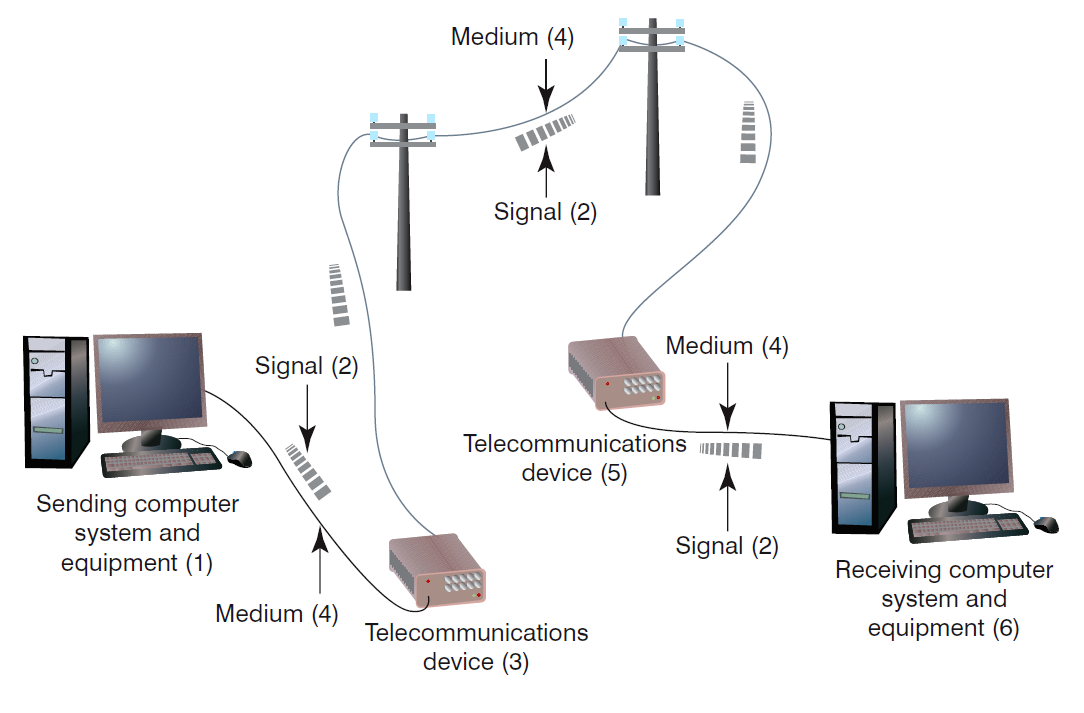
\includegraphics[width=0.75\textwidth]{chapter06/telecommunications_system.png}
			\end{center}
			The speed at which information is transmitted is measured in bits per second (bps), and typically range from thousands (Kbps) to millions (Mbps) to billions (Gbps).
			\begin{sidenote}{Synchronous vs Asynchronous}
				\begin{description}[nosep]
					\item[Synchronous] The receiver gets the message almost instantaneously when it is sent. For example, phone communication.
					\item[Asynchronous] There is a measurable delay between the sending and receiving of the message. For example, sending a message through the post office or via email.
				\end{description}
			\end{sidenote}
			\begin{definition}{Channel Bandwidth}
				The rate at which data is exchanged over a communications channel, usually measured in bits per second.

				The broader the bandwidth, the more information can be exchanged at one time.
				\begin{description}[nosep]
					\item[Broadband communications] A telecommunications system in which a very high rate of data exchange is possible.
					\item[Narrowband communications] A telecommunications system that supports a much lower rate of data exchange than broadband.
				\end{description}
			\end{definition}
			Transmission media can be divided into two types:
			\begin{indentparagraph}
				\begin{description}[nosep]
					\item[Guided Transmission Media] Communication signals are guided along a solid medium
					\item[Wireless Transmission Media] Communication signals are broadcast over airwaves as a form of electromagnetic radiation. 
				\end{description}
			\end{indentparagraph}
			\subsection{Guided Transmission Media Types}
				\begin{sidenote}{Guided Media Types}
					\begin{center}
						\begin{tblr}{colspec={>{\raggedright}X[2]>{\raggedright}X[3]>{\raggedright}X[3]>{\raggedright}X[3]}, row{even}={white}, row{1}={font=\bfseries}, column{1}={font=\bfseries}}
							Media Types & Description & Advantages & Disadvantages\\
							\midrule
							Twisted-pair wire & Twisted pairs of copper wires, shielded or unshielded & Used for telephone service; widely available & Transmission speed and distance limitations\\
							Coaxial Cable & Inner conductor wire surrounded by insulation & Cleaner and faster data transmission than twisted-pair wire & More expensive than twisted-pair wire\\
							Fibre-optic cable & Many extremely thin strands of glass bound together in a sheathing; uses light beams to transmit signals & Diameter of cable is much smaller than coaxial; less distortion of signal; capable of high transmission rates & Expensive to purchase and install\\
							Broadband over power lines & Data is transmitted over standard high-voltage power lines & Can provide Internet service to rural areas where cable and phone service may be non-existent & Can be expensive, and may interfere with amateur radios, police and fire communications 
						\end{tblr}
					\end{center}
				\end{sidenote}
			\subsection{Wireless Transmission Media Types}
				\subsubsection{Microwave Transmission}
					\begin{definition}{Microwave Transmission}
						High frequency (300 MHz to 300 GHz) signal sent through the air. Terrestrial (earth-bound) microwaves are transmitted by \concept{line-of-sight devices}. Can carry thousands of channels at the same time.
					\end{definition}
					\begin{sidenote}{Communications Satellites}
						A communications satellite also operates in the microwave frequency range. The advantage is that is can receive and broadcast over large geographic regions.
						\begin{description}
							\item[Geostationary Satellite] Orbits the Earth directly over the Equator, positioned a large distance above the Earth, so that it appears stationery. Three such satellites, spaced at even intervals, can span the entire Earth. Can be accessed using a dish antenna aimed at the spot in the sky where the satellite hovers.
							\item[Low Earth Orbit Satellite (LEO)] Employs many satellites, each in a circular orbit at an altitude of a few hundred kilometres.
							\item[Very Small Aperture Terminal (VSAT)] A two-way satellite ground station with a dish antenna smaller than three metres in diameter.
						\end{description}
					\end{sidenote}
				\subsubsection{5G Wireless Communication}
					\begin{sidenote}{Wireless Communication Generations}
						\begin{description}
							\item[First Generation (1G)] Originated in the 1980s, based on analogue communications.
							\item[Second Generation (2G)] Early 1990s, fully digital. Phone conversations encrypted, mobile phone usage expanded, \concept{short message services (SMS)} introduced.
							\item[Third Generation (3G)] Supports wireless voice and broadband speed data communications in a mobile environment at speeds of 2 to 4 Mbps. Mobile video, mobile e-commerce, location-based services, mobile gaming, downloading and playing music.
							\item[Fourth Generation (4G)] More advanced versions of enhanced multimedia, smooth streaming video, universal access and portability. 20 times the speed of 3G.
							\item[Fifth Generation (5G)] Higher data transmission rates, lower power consumption, higher connection reliability, increased geographic coverage, lower infrastructure costs. 
						\end{description}
					\end{sidenote}
				\subsubsection{Wi-Fi}
					\begin{definition}{Wi-Fi}
						A medium-range wireless telecommunications technology brand owned by the Wi-Fi alliance.

						The user's device has a wireless adapter that translates data into a radio signal and transmits it using an antenna. A \concept{wireless access point}, which consists of a transmitter with an antenna, receives the signal and decodes it.
					\end{definition}
				\subsubsection{Near Field Communication}
					\begin{definition}{Near Field Communication (NFC)}
						A very short-range wireless connectivity technology designed for credit cards, consumer electronics, and smartphones.

						Works with 2 devices, that need to be in proximity (touching, or a few centimetres apart). Exchange the necessary communications parameters to enable Bluetooth, Wi-Fi, or other communications between the devices. Establishes a \concept{peer-to-peer network}.
					\end{definition}
				\subsubsection{Bluetooth}
					\begin{definition}{Bluetooth}
						A wireless communication specification that describes how smartphones, computers, printers, and other devices can be interconnected over distances of a few meters at a rate of about 2 Mbps.
					\end{definition}
				\subsubsection{Ultra Wideband}
					\begin{definition}{Ultra Wideband (UWB)}
						A form of short-range communication that employs extremely short electromagnetic pulses lasting 50 to 1000 picoseconds that are transmitted over a broad range of radio frequencies or several gigahertz.

						Advantages: A high throughput rate, the ability to transmit undetected, and impervious to interception or jamming, and a lack of interference with current communications services.
					\end{definition}
				\subsubsection{Infrared Transmission}
					\begin{definition}{Infrared Transmission (IR)}
						A mode of transmission that sends signals through the air via light waves at a frequency of 300 GHz and above. Requires line-of-sign transmission, and short distances.
					\end{definition}
			\pagebreak
			\subsection{Telecommunications Hardware}
				\subsubsection{Modems}
					\begin{definition}{Analogue Signal}
						A variable signal continuous in both time and amplitude, so that any small fluctuations in the signal are meaningful.
					\end{definition}
					\begin{definition}{Digital Signal}
						A signal that represents bits.
					\end{definition}
					\begin{definition}{Modem (Modulator/Demodulator)}
						A telecommunications hardware device that modulates and demodulates communications signals, so they can be transmitted over the communication media.
						\begin{description}
							\item[Modulation] Translating data from digital to analogue.
							\item[Demodulation] Translating data from analogue to digital. 
						\end{description}
					\end{definition}
				\subsubsection{Multiplexers}
					\begin{definition}{Multiplexer}
						A device that encodes data from two or more data sources onto a single communications channel, this reducing their number of communications channels needed and therefore lowering telecommunications costs.
					\end{definition}
				\subsubsection{Front-End Processors}
					\begin{definition}{Front-End Processor}
						A special-purpose computer that managers communications to and from a computer system serving hundreds or even thousands of users.
					\end{definition}
				\subsubsection{Private Branch Exchange}
					\begin{definition}{Private Branch Exchange (PBX)}
						A telephone switching exchange that serves a single organisation.

						Enables users to share a certain number of outside lines (\concept{trunk lines}) to make telephone calls to people outside the organisation.
					\end{definition}
				\subsubsection{Switches, Bridges, Routers, and Gateways}
					\begin{definition}{Switch}
						A telecommunications device that uses the physical device address in each incoming message on the network, to determine to which output port it should forward the message, to reach another device on the same network.
					\end{definition}
					\begin{definition}{Bridge}
						A telecommunications device that connects one LAN to another LAN that uses the same telecommunications protocol.
					\end{definition}
					\begin{definition}{Router}
						A telecommunications device that forwards data packets across two or more distinct networks towards their destinations, through a process known as \concept{routing}.
					\end{definition}
					\begin{definition}{Gateway}
						A telecommunications device that serves as an entrance to another network.
					\end{definition}

	\vbox{\rulechapterend}
\end{document}